\documentclass{standalone}
\usepackage{tikz}
\usepackage{pgfplots}
\begin{document}
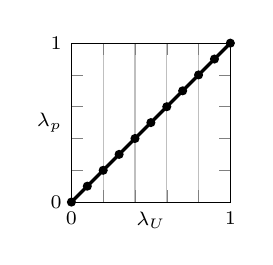
\begin{tikzpicture}[font=\scriptsize]

\begin{axis}[
      xmin=0, xmax=1,
      ymin=0, ymax=1,
      width=3.6cm,
      height=3.6cm,
      xlabel=$\lambda_U$,
      ylabel=$\lambda_p$,
      xlabel near ticks,
      ylabel near ticks,
      %xmin=0, xmax=1,
      %ymin=0, ymax=15,
      xticklabels={,0,,,,,1},
      yticklabels={,0,,,,,1},
      ticklabel style={font=\scriptsize},
      xmajorgrids,
      y label style={at={(axis description cs:0,.5)},rotate=-90,anchor=east},
      x label style={at={(axis description cs:0.5,0.0)},anchor=north}]
   
   \addplot
      plot[color=black,very thick,mark options={color=green},mark options={scale=0.5}]
      coordinates {
         (0.0,0.0)
         (0.1,0.1)
         (0.2,0.2)
         (0.3,0.3)
         (0.4,0.4)
         (0.5,0.5)
         (0.6,0.6)
         (0.7,0.7)
         (0.8,0.8)
         (0.9,0.9)
         (1.0,1.0)
      };

\end{axis}

\end{tikzpicture}
\end{document}
